\chapter{Design \& Specification}

This section will present an abstract view of how the system works.
The project is split into 3 main components - the web app , the backend and another external backend exclusively for running user code.

\section{Use cases}
\begin{figure}[H]
  \centering

	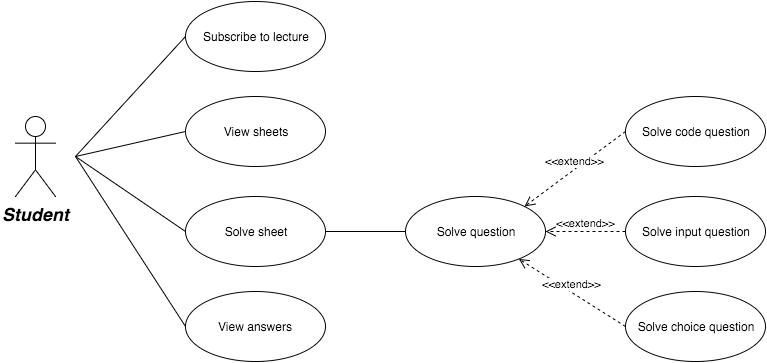
\includegraphics[width=\textwidth,height=\textheight,keepaspectratio]{cases}
	\caption{Use cases for students}
\end{figure}

\begin{figure}[H]
  \centering

	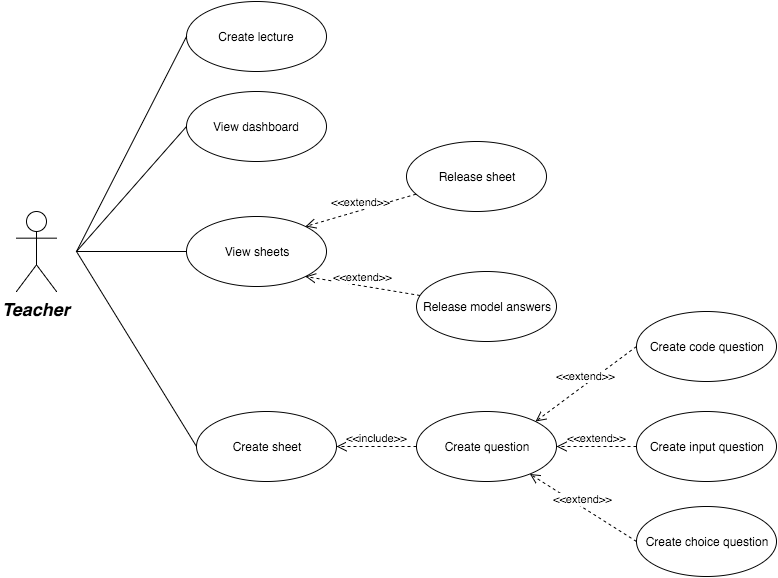
\includegraphics[width=\textwidth,height=\textheight,keepaspectratio]{cases2}
	\caption{Use cases for teachers}
\end{figure}

\section{System architecture}
\subsection{Backend}
The backend provides a simple HTTP REST API that the front end can use. It is built in such a way that the front-end is a replaceable component and may be updated or switched during further development , data is encoded as JSON unless the payload represents one single value (like a number) in which case it is not wrapped in a JSON object.

The backend provides all the data needed for the application to render what it needs to show , as well as allowing the client to POST data to the server to update resources.

The endpoints of the API which may return private information have safeguards such that they will not expose information that the user should not be seeing - this is achieved by checking the user that is authenticated. This is to conform to Data Protection laws that impose limit data access where possible.

Authentication works via session cookies , this is implemented using the Devise ruby gem as reference in section \ref{libs}. If the user is not logged in he is redirected to the login/signup page.

The database itself is a PostgresSQL database, it resides on the same server as this backend and is protected with username/password authentication.

\subsection{Code running backend}
The other backend is solely responsible for running arbitrary code written by users , this acts as a security measure in case a malicious agent manages to escape the container and compromise the server.

The endpoint this server exposes takes a piece of code , the language it's written in and a map of inputs and outputs. The code is written to a temporary file in a temporary folder. Then , depending on the language , a docker instance with the right runtime is started - when creating this instance , the temporary folder is mounted (mapped) to the docker instance inside the container's root drive. Then the file is executed inside the virtual machine with all the inputs , if the outputs generated match the given model answers then the API returns true ; else false. 

Since the container only has access to the temporary folder where the code file is , it cannot harm the outer filesystem. In fact , deleting the root folder inside the container would only delete the code file and nothing else.
If the code does not compile or there is a runtime error , the sever will wrap the error in a JSON object and return it to the main backend which will show it to the user.

\subsection{Diagram}

\section{User interface}
Since the user's are assumed to be somewhat technically savvy , the application takes some liberties with having a limited amount of help and information banners since it works similarly to other website the target audience is familiar with ( markdown used in websites like Stackoverflow \cite{stackoverflow} ).
Overall the application is meant to have a flat design that looks good on any resolution and is not based on bitmaps but rather on shapes - as they are more versatile and do not need to be updated as often.
Each lecture has a colour chosen by the teacher and shows up throughout the user interface so the user knows which lecture they are looking at and provides a sense of cohesion to the application.


\section{Security}
Because the project allows users to input and run arbitrary code it is important to have proper security in place. There are four layers of security for running code:
\begin{itemize}
\item Users can only run non-native code , currently Python and Java
\item 	All user code runs in secure Docker containers
\item	Containers are contained in a separate server
\item User code runs as non-root within the container
\end{itemize}
Because the code execution server and the database/main server are separate , even if a malicious agent used a vulnerability to break out of the container, he may not access any information or maliciously disrupt server operations.

Docker is used to create containers to safetly run arbitrary code , outside of a container being basically a virtual machine Docker added extra security features \cite{dockersecurity} such as restricting the capabilities of the linux kernel , namespaces and control groups.



\section{Database}
There is one database in use which contains all the information relevant to the system , it is located on the same server as the backend ; further in the report you will find some notes on how this can be improved and why.
The database schema is very important since changing it could break parts of the system , it was important to chose a structure that would not drastically change later in the development cycle.
Below is the structure of the tables in the system

\subsubsection{Lecture table}
This table contains all the lectures created

\begin{itemize}
	\item \textit{\textbf{Name}} The name of the lecture , there may be multiple lectures with the same name
	\item  \textit{\textbf{Author}} The teacher who created the lecture , can be any user of the system
	\item  \textit{\textbf{Color}} A Hex , RGB or any valid HTML colour , the current UI allows the teacher to choose a colour from a predefined set. It is used in a number of pages , often used to style all controls on the page - such as buttons or tabs	
\end{itemize}

\subsubsection{Sheet table}
This table contains all the sheets created

\begin{itemize}
	\item  \textit{\textbf{Name}} The name of the sheet
	\item  \textit{\textbf{Lecture ID}} The ID of the lecture this sheet belongs to
	\item  \textit{\textbf{Live}} A boolean that represents whether the students who are subscribed to the lecture can see this sheet ( the teacher can use this to choose when to let the students start completing the sheet)
	\item  \textit{\textbf{Released}} A boolean value that represents if the model answers are released (and the user may no longer change his answers)
\end{itemize}

\subsubsection{Question table}
This table contains all the questions created

\begin{itemize}
	\item  \textit{\textbf{Title}} The body of the question as Markdown formatted text ( stored as plaintext)
	\item  \textit{\textbf{Sheet ID}} The ID of the sheet this question belongs to
	\item  \textit{\textbf{Data}} JSON that provides metadata needed to render the question
	\item  \textit{\textbf{Type}} An integer that defines the type of question
	\item  \textit{\textbf{Correct Answer}} A JSON object that defines metadata needed to compute whether the answer is correct or not	
	\item  \textit{\textbf{Model Answer}} A string that represents an example answer
\end{itemize}

\subsubsection{Answer table}
This table contains all the answers created

\begin{itemize}
	\item  \textit{\textbf{Data}} A plaintext representation of the student's answer
	\item  \textit{\textbf{Question ID}} The question that is answered
	\item  \textit{\textbf{User ID}} The ID of the student who created this answer
	\item  \textit{\textbf{Result}} Plaintext field , used to store the cached computed result of the question.
\end{itemize}

\subsubsection{Statistic table}
This table contains all the statistics created when students answer questions

\begin{itemize}
	\item  \textit{\textbf{Answer ID}} The ID of the answer this statistic is about
	\item  \textit{\textbf{Data}} JSON that contains relevant statistical information about the action
	\item  \textit{\textbf{Kind}} The type of statistic this represents
\end{itemize}



\subsubsection{Subscription table}
This table contains all the subscriptions

\begin{itemize}
	\item  \textit{\textbf{Lecture ID}} The ID of the lecture the user is subscribed to
	\item  \textit{\textbf{User ID}} The ID of the user subscribing to the lecture
\end{itemize}





















